\documentclass[journal,10pt,twocolumn]{article}
\usepackage{graphicx}
\usepackage[margin=0.5in]{geometry}
\usepackage[cmex10]{amsmath}
\usepackage{array}
\usepackage{booktabs}
\title{\textbf{Conic Assignment}}
\author{Bhavani Kanike}
\date{October 2022}

\providecommand{\norm}[1]{\left\lVert#1\right\rVert}
\providecommand{\abs}[1]{\left\vert#1\right\vert}
\let\vec\mathbf
\newcommand{\myvec}[1]{\ensuremath{\begin{pmatrix}#1\end{pmatrix}}}
\newcommand{\mydet}[1]{\ensuremath{\begin{vmatrix}#1\end{vmatrix}}}
\providecommand{\brak}[1]{\ensuremath{\left(#1\right)}}

\begin{document}

\maketitle
\paragraph{\textit{Problem Statement} \\\\- On the ellipse 4$x^2$ + 9$y^2$ = 1, the points at which the tangents are parallel to the line 8x = 9y are . }

\section*{\large Solution}

\section*{\large Construction}

\begin{figure}[h]
\centering
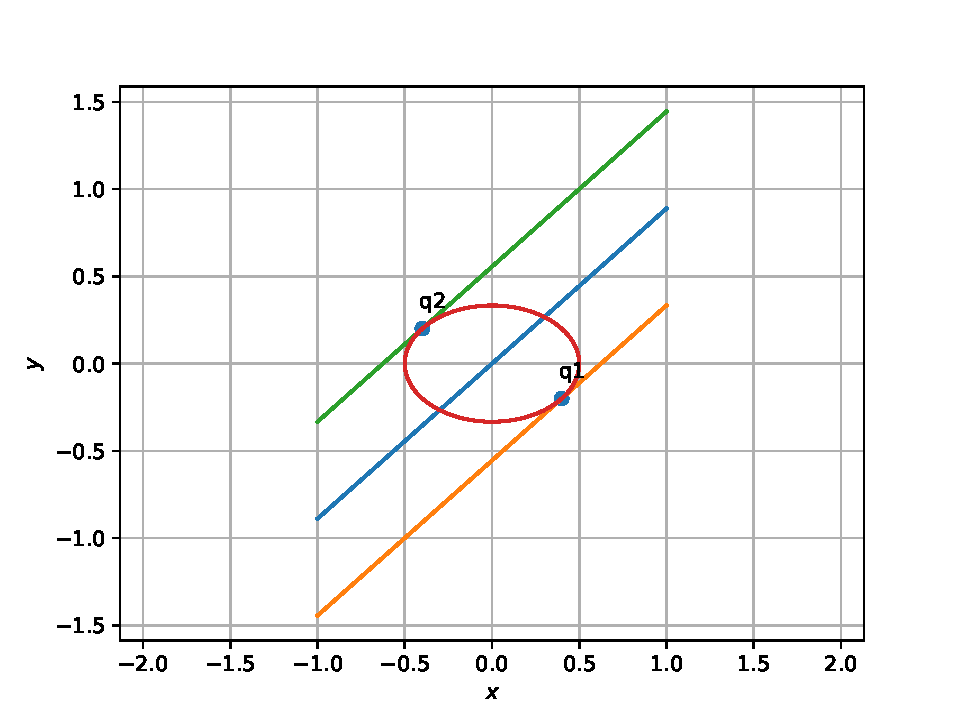
\includegraphics[width=1\columnwidth]{conic1.pdf}
\caption{Figure}
\label{fig:triangle}
\end{figure}

The dimensions of the figure is taken as below\\
{
\setlength\extrarowheight{2pt}
\centering
	\begin{tabular}{|c|c|}
	\hline
	\textbf{symbol}&\textbf{value}\\
	\hline
	u &$\myvec{0\\0}$\\
	\hline
	a&1/4\\
	\hline
	b&1/9\\
	\hline
	V&$\myvec{1/4&0\\0&1/9}$\\
	\hline
	n&$\myvec{8\\-9}$\\
	\hline
\end{tabular}
}\\\\

	$\boldsymbol{Given :}$ Ellipse Equation\\
\begin{equation}
	4x^2 + 9y^2 = 1
\end{equation}
 Line Equation :	8x = 9y\\\\
 The standard equation of the conic is given by \\
\begin{equation}
	\vec{x}^{\top}\vec{V}\vec{x}+2\vec{u}^{\top}\vec{x}+f=0
\end{equation}
 
 The given circle can be expressed as conics with \\Prameters
\begin{equation}
	\lambda_1 = \frac{1}{4} , \lambda_2 = \frac{1}{9}
\end{equation}
\begin{equation}
	\vec{V} = \myvec{\lambda_2&0\\0&\lambda_1} = \myvec{1/9&0\\0&1/4} , \vec{u} = \myvec{0\\0} , f = -\lambda_1\lambda_2 = \frac{1}{36}
\end{equation}
\\
To find the Points on ellipse which forms a tangent parallel to the line 
\begin{equation}
	8x - 9y = 0
\end{equation}
The points are given by the following equation:
\begin{equation}
	\vec{q} = \vec{V}^{-1}(k_i\vec{n}-\vec{u})
\end{equation}
And the intermediate parameters are given by 
\begin{equation}
	k_i = \pm\sqrt{\frac{\vec{u}^T\vec{V}^{-1}\vec{u}-f}{\vec{n}\vec{V}^{-1}\vec{n}}}
\end{equation} 
$\vec{n}$ is the normal vector of tangent from point $\vec{q1}$ and $\vec{q2}$ 
\begin{equation}
	\vec{n} = \myvec{8\\-9}
\end{equation}
Now to obtain the values of $k_1$ and $k_2$ , substitute $\vec{n}$ in equation 7
\begin{equation}
	V^{-1} = \myvec{9&0\\0&4}
\end{equation}

\begin{equation}
	k_1 = \sqrt{\frac{\myvec{0\\0}^T\myvec{9&0\\0&4}\myvec{0\\0}}{\myvec{8\\-9}^T\myvec{9&0\\0&4}\myvec{8\\-9}}}
\end{equation}
\begin{equation}
	k_1 = 0.0055
\end{equation}
\begin{equation}
	k_2 = - \sqrt{\frac{\myvec{0\\0}^T\myvec{9&0\\0&4}\myvec{0\\0}}{\myvec{8\\-9}^T\myvec{9&0\\0&4}\myvec{8\\-9}}}
\end{equation}
\begin{equation}
	k_2 = -0.0055
\end{equation}
\begin{equation}
	\vec{q_1} = \myvec{9&0\\0&4}(k_1*\myvec{8\\-9} - \myvec{0\\0})
\end{equation}
\begin{equation}
	\vec{q_1} = \myvec{ 0.4\\-0.2}
\end{equation}
\begin{equation}
	\vec{q_2} = \myvec{9&0\\0&4}(k_2*\myvec{8\\-9} - \myvec{0\\0})
\end{equation}
\begin{equation}
	\vec{q_2} = \myvec{-0.4\\0.2}
\end{equation}

\end{document}